\chapter{Results}

% pre-figure explanation
  We rendered the resulting behaviors produced by controllers trained on aforementioned reward functions and environments into images or frames.
  Combining the frames generated for each of the 1000 timesteps and setting as 60 frames per second resulted in 33.35 second videos.
  The time-lapses presented in Figures \ref{fig:manual_trajectory_body_speed_0}, \ref{fig:manual_trajectory_strict_body_speed_1}, \ref{fig:manual_trajectory_not_strict_body_speed_1}, \ref{fig:fifty_fifty_body_speed_0}, and \ref{fig:fifty_fifty_body_speed_1} were created by sampling every $300$ frames within the last 30 seconds of the video.
  The frames' sequential order is from the top left to the bottom right.
  The camera is locked to follow the pigeon's body.
  % 60/5 * [10] = 300

% summary of the results
  % We summarize the behaviors exhibited by each experiment as stated in the previous chapter.

  % The pigeon model with a static body whose controller was trained using $r_{head\_stable\_manual\_reposition\_strict\_angle}$ managed to keep its head stationary as expected.

  % The pigeon model with the body speed of 1 whose controller was trained using $r_{head\_stable\_manual\_reposition\_strict\_angle}$
    % initially struggled to control its head in a specific pattern or position.
    % However, after 5 seconds, it managed to align the head within the radius $max\_offset$ around the manually set position $T$, resulting in a generation of trajectory that depicts a pattern of thrust and hold phases.
    % The final 5 seconds of the footage depicts the head and the limbs getting stuck on the topside of the body.

  % The pigeon model with the body speed of 1 whose controller was trained using $r_{head\_stable\_manual\_reposition}$ produced similar results to the previous experiment, with the exception of the overall performance.
  % Due to the less strict definition of the reward function, it generated a trajectory that resulted in the acquirement of larger return, and as a result, a better performance in producing the desired head-bobbing behavior.
  % In particular, the timespan of the head following the manually-defined trajectory was longer than those seen in the previous experiment.

  % 4. head wiggles relatively in the same position; similar to the baseline counterpart
  % 5. head gradually leans down and backwards; as if it was following the stationary object

  \begin{figure}[H]
      \centering
      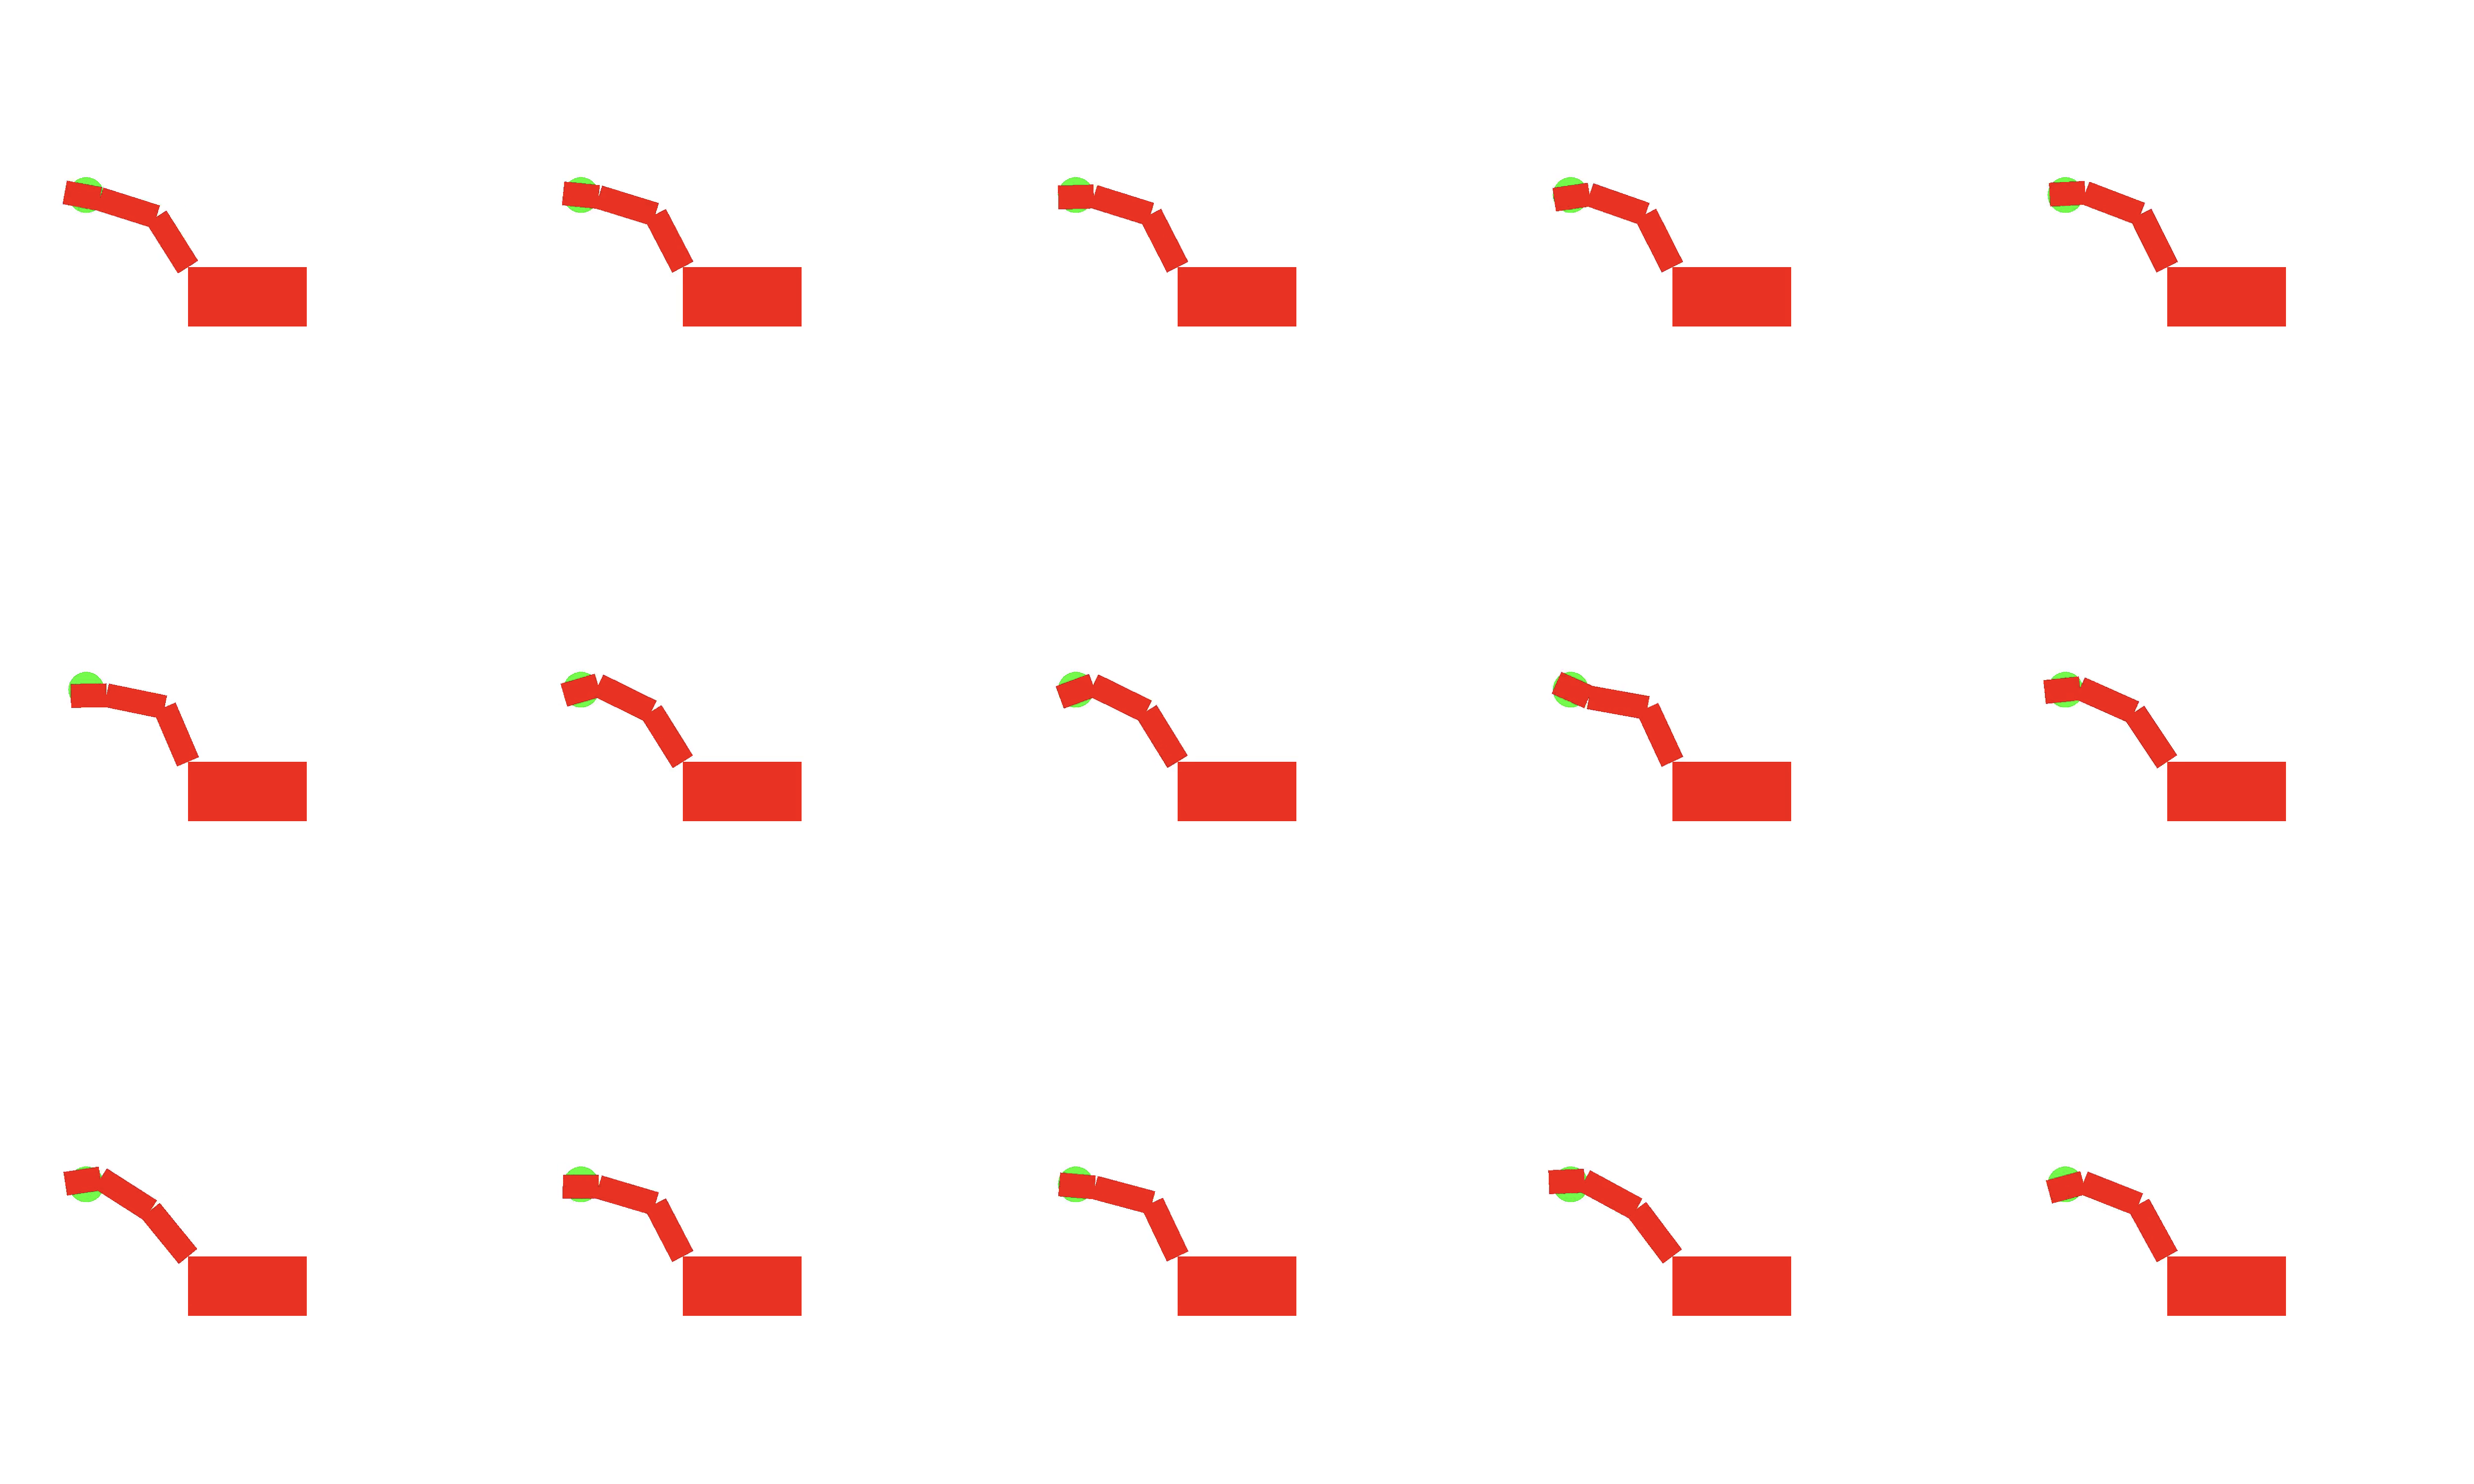
\includegraphics[width=1\textwidth]{figures/frames/frames_001.png}
      \caption{Control of a pigeon model with a static body trained on $r_{head\_stable\_manual\_reposition\_strict\_angle}$ with $max\_offset = 0.5$. The green circle indicate the margin of error around the target head location defined by $max\_offset$.}
      \label{fig:manual_trajectory_body_speed_0}
  \end{figure}

  \begin{figure}[H]
      \centering
      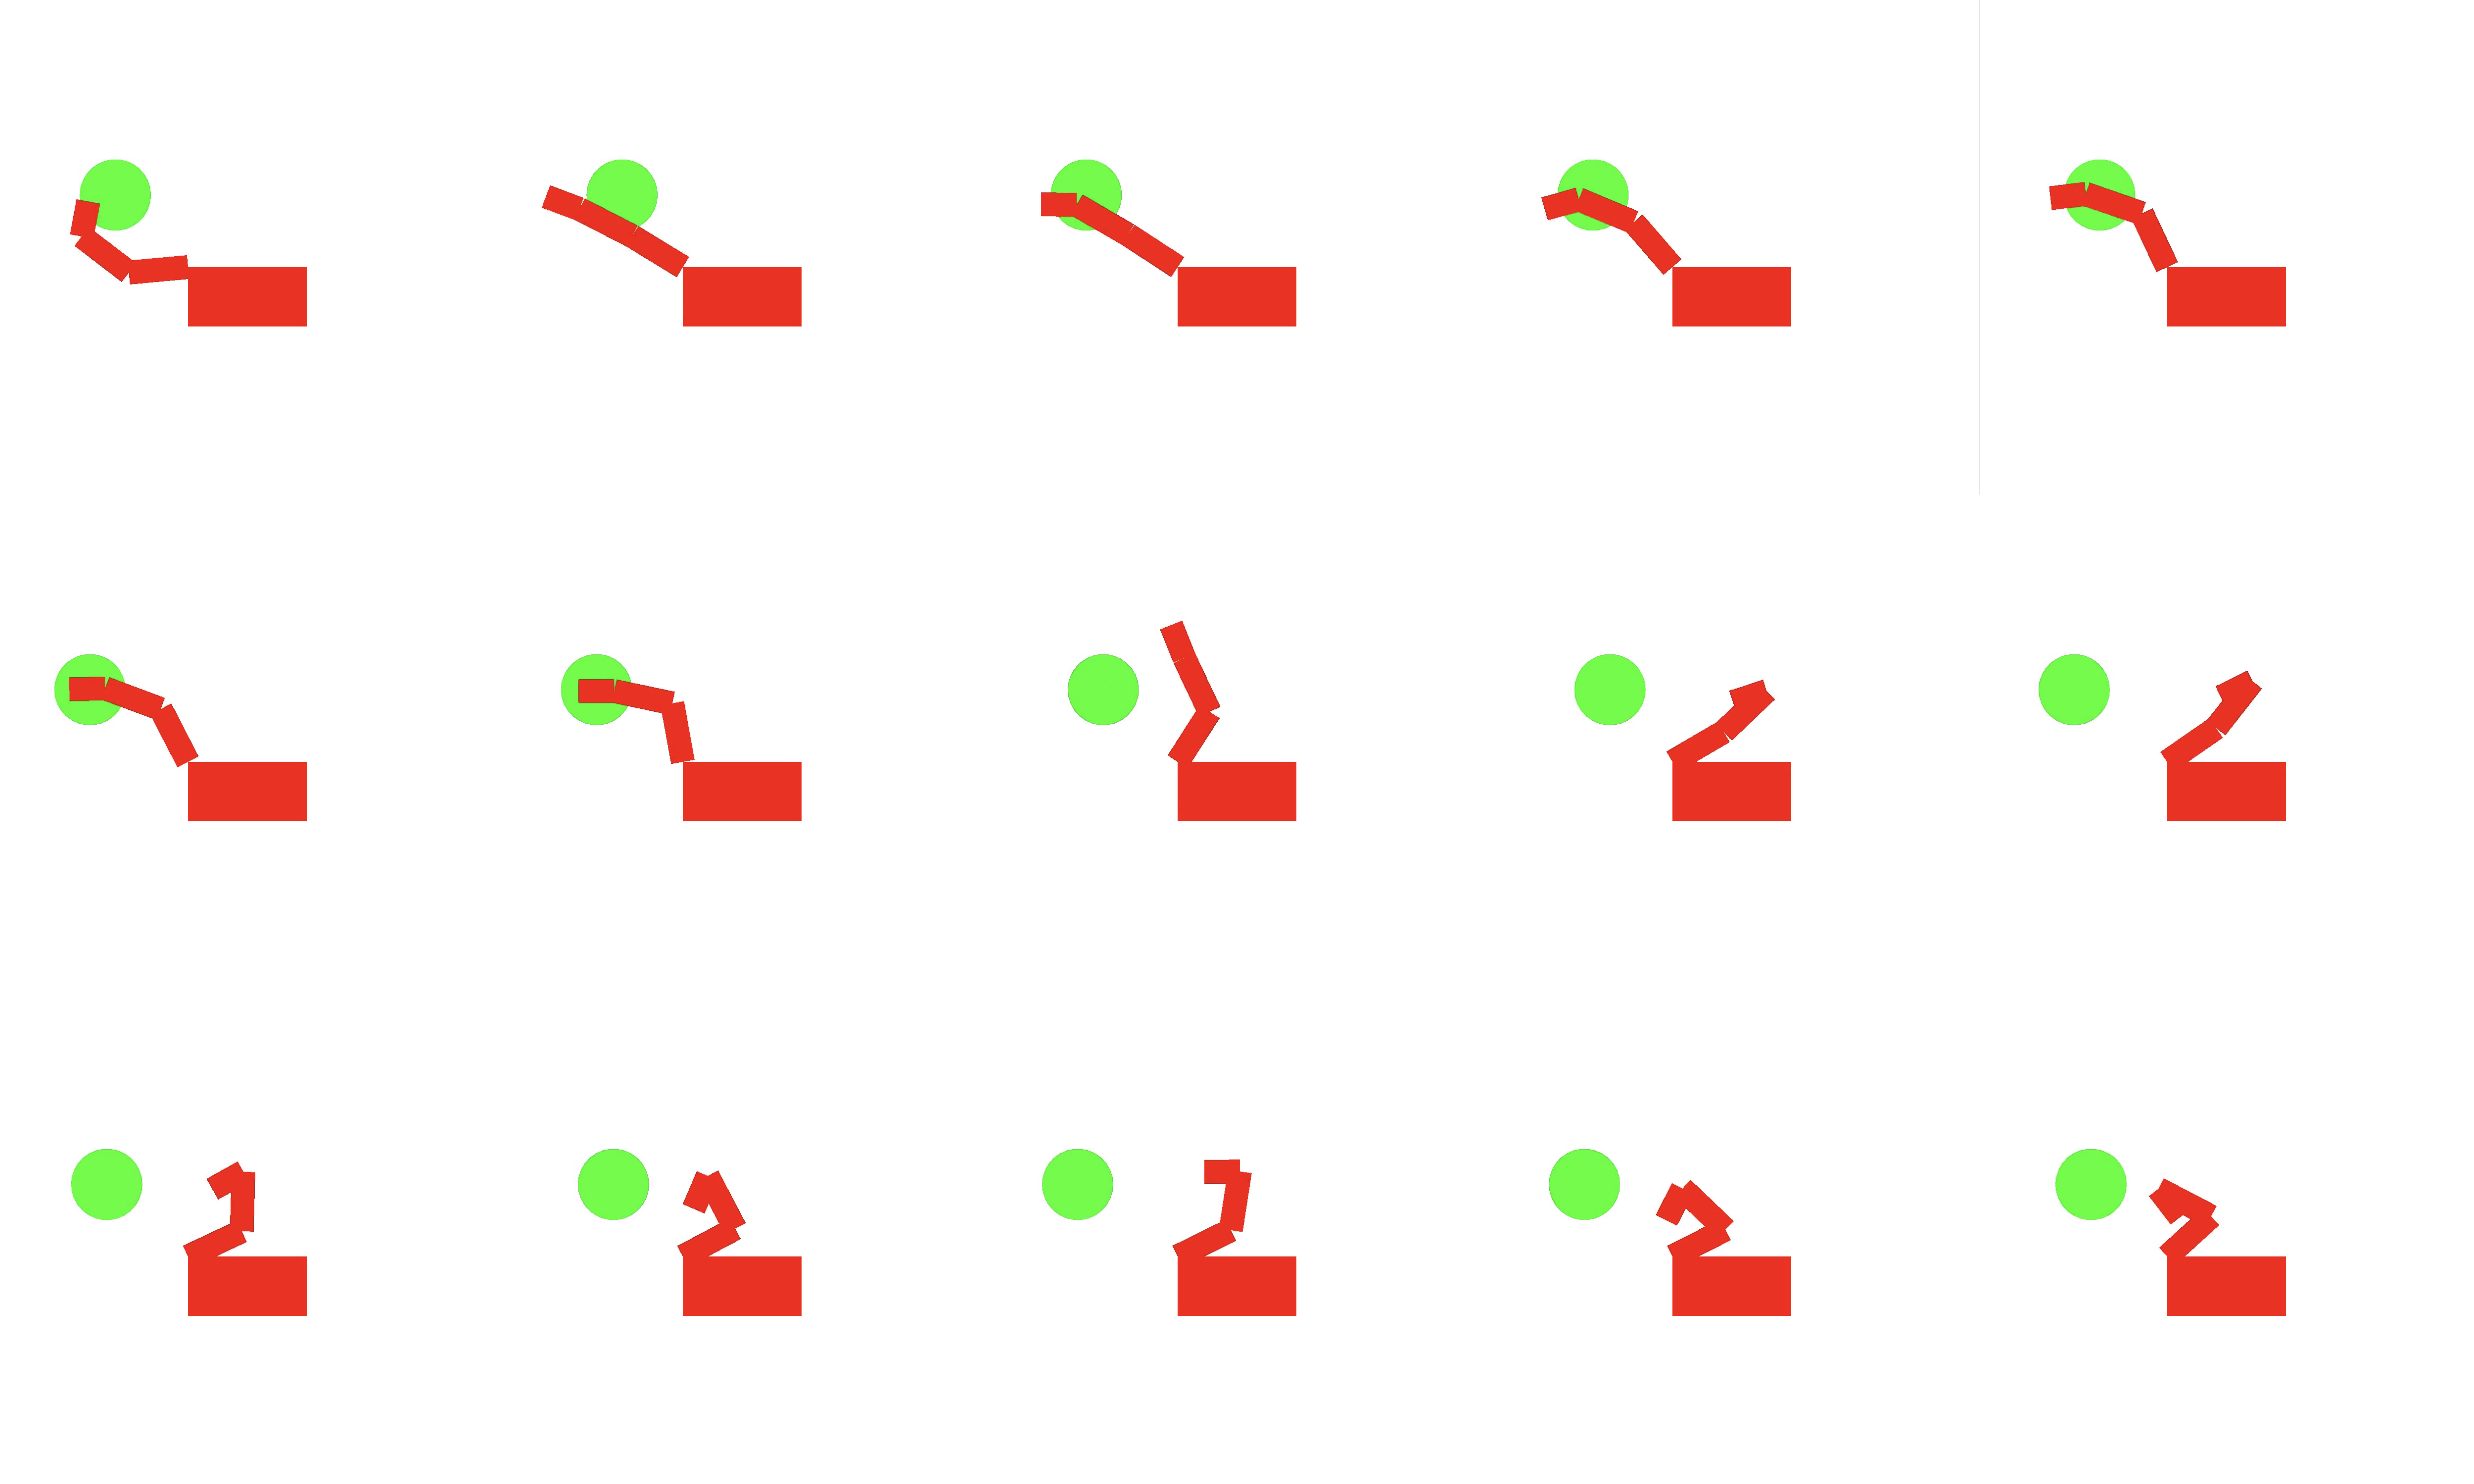
\includegraphics[width=1\textwidth]{figures/frames/frames_002.png}
      \caption{Control of a pigeon model with the body speed of 1 trained on $r_{head\_stable\_manual\_reposition\_strict\_angle}$ with $max\_offset = 1.0$. The green circle indicate the margin of error around the target head location defined by $max\_offset$.}
      \label{fig:manual_trajectory_strict_body_speed_1}
  \end{figure}

  \begin{figure}[H]
      \centering
      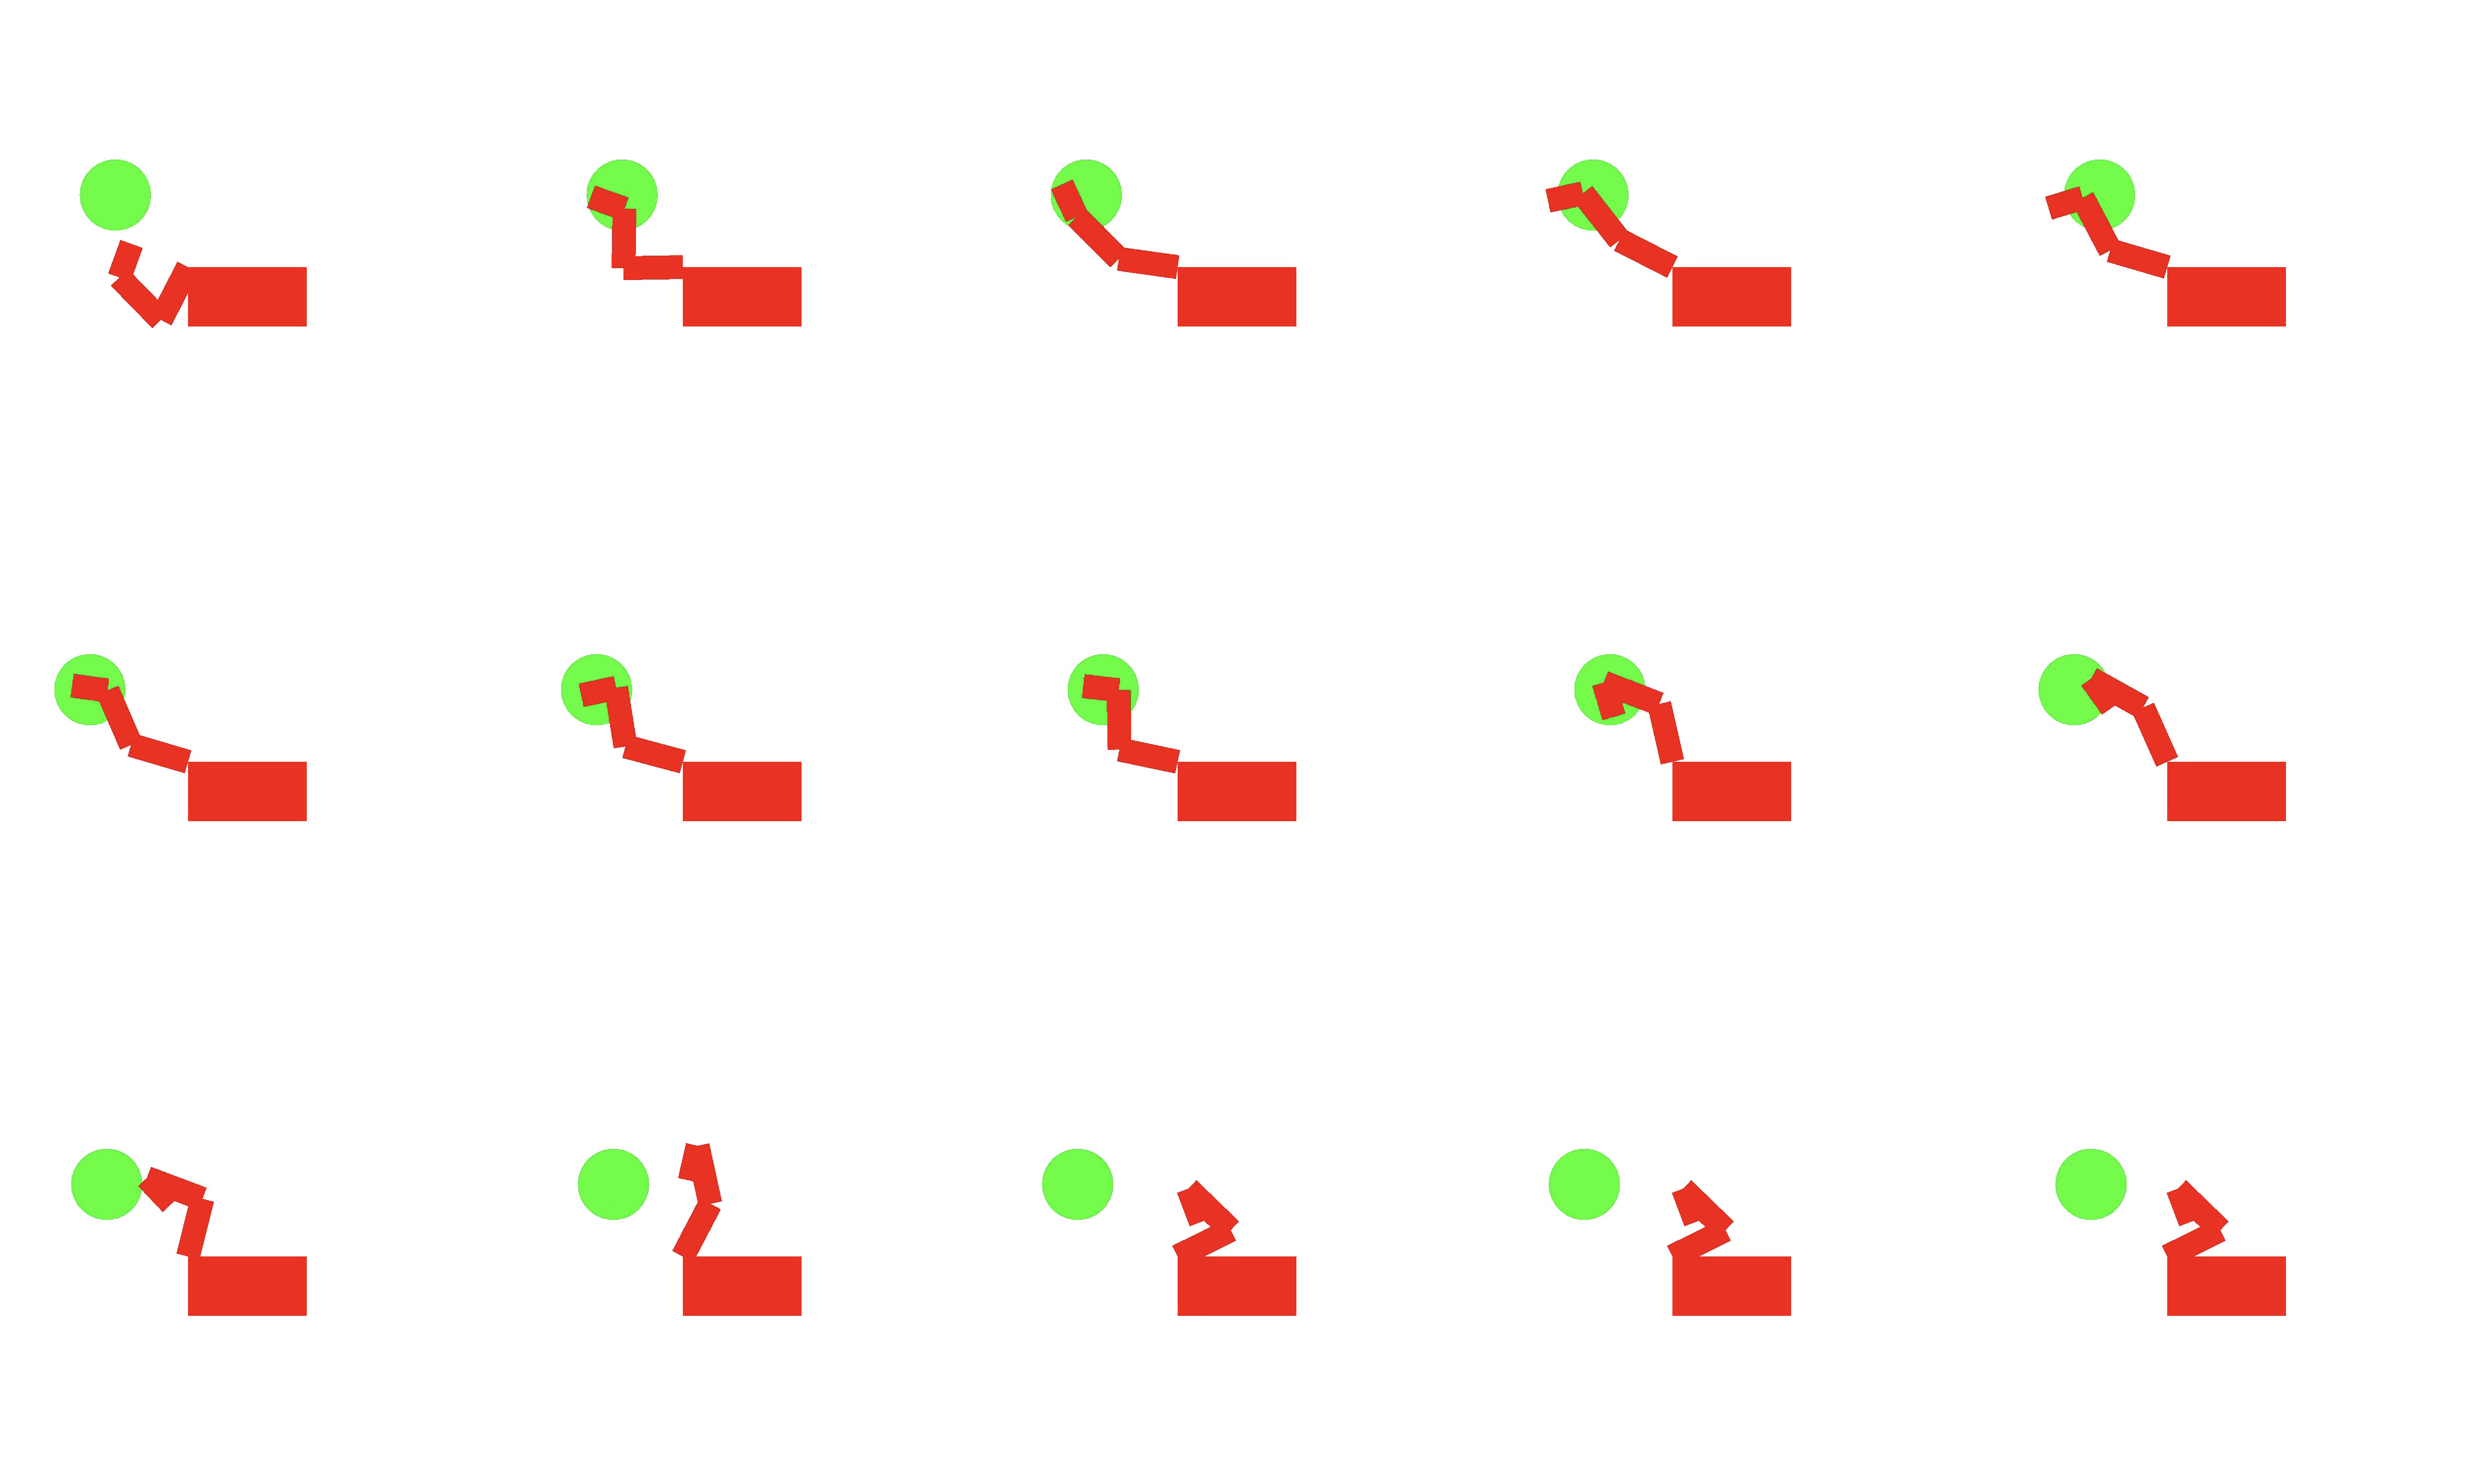
\includegraphics[width=1\textwidth]{figures/frames/frames_003.png}
      \caption{Control of a pigeon model with the body speed of 1 trained on $r_{head\_stable\_manual\_reposition}$ with $max\_offset = 1.0$. The green circle indicate the margin of error around the target head location defined by $max\_offset$.}
      \label{fig:manual_trajectory_not_strict_body_speed_1}
  \end{figure}

  \begin{figure}[H]
      \centering
      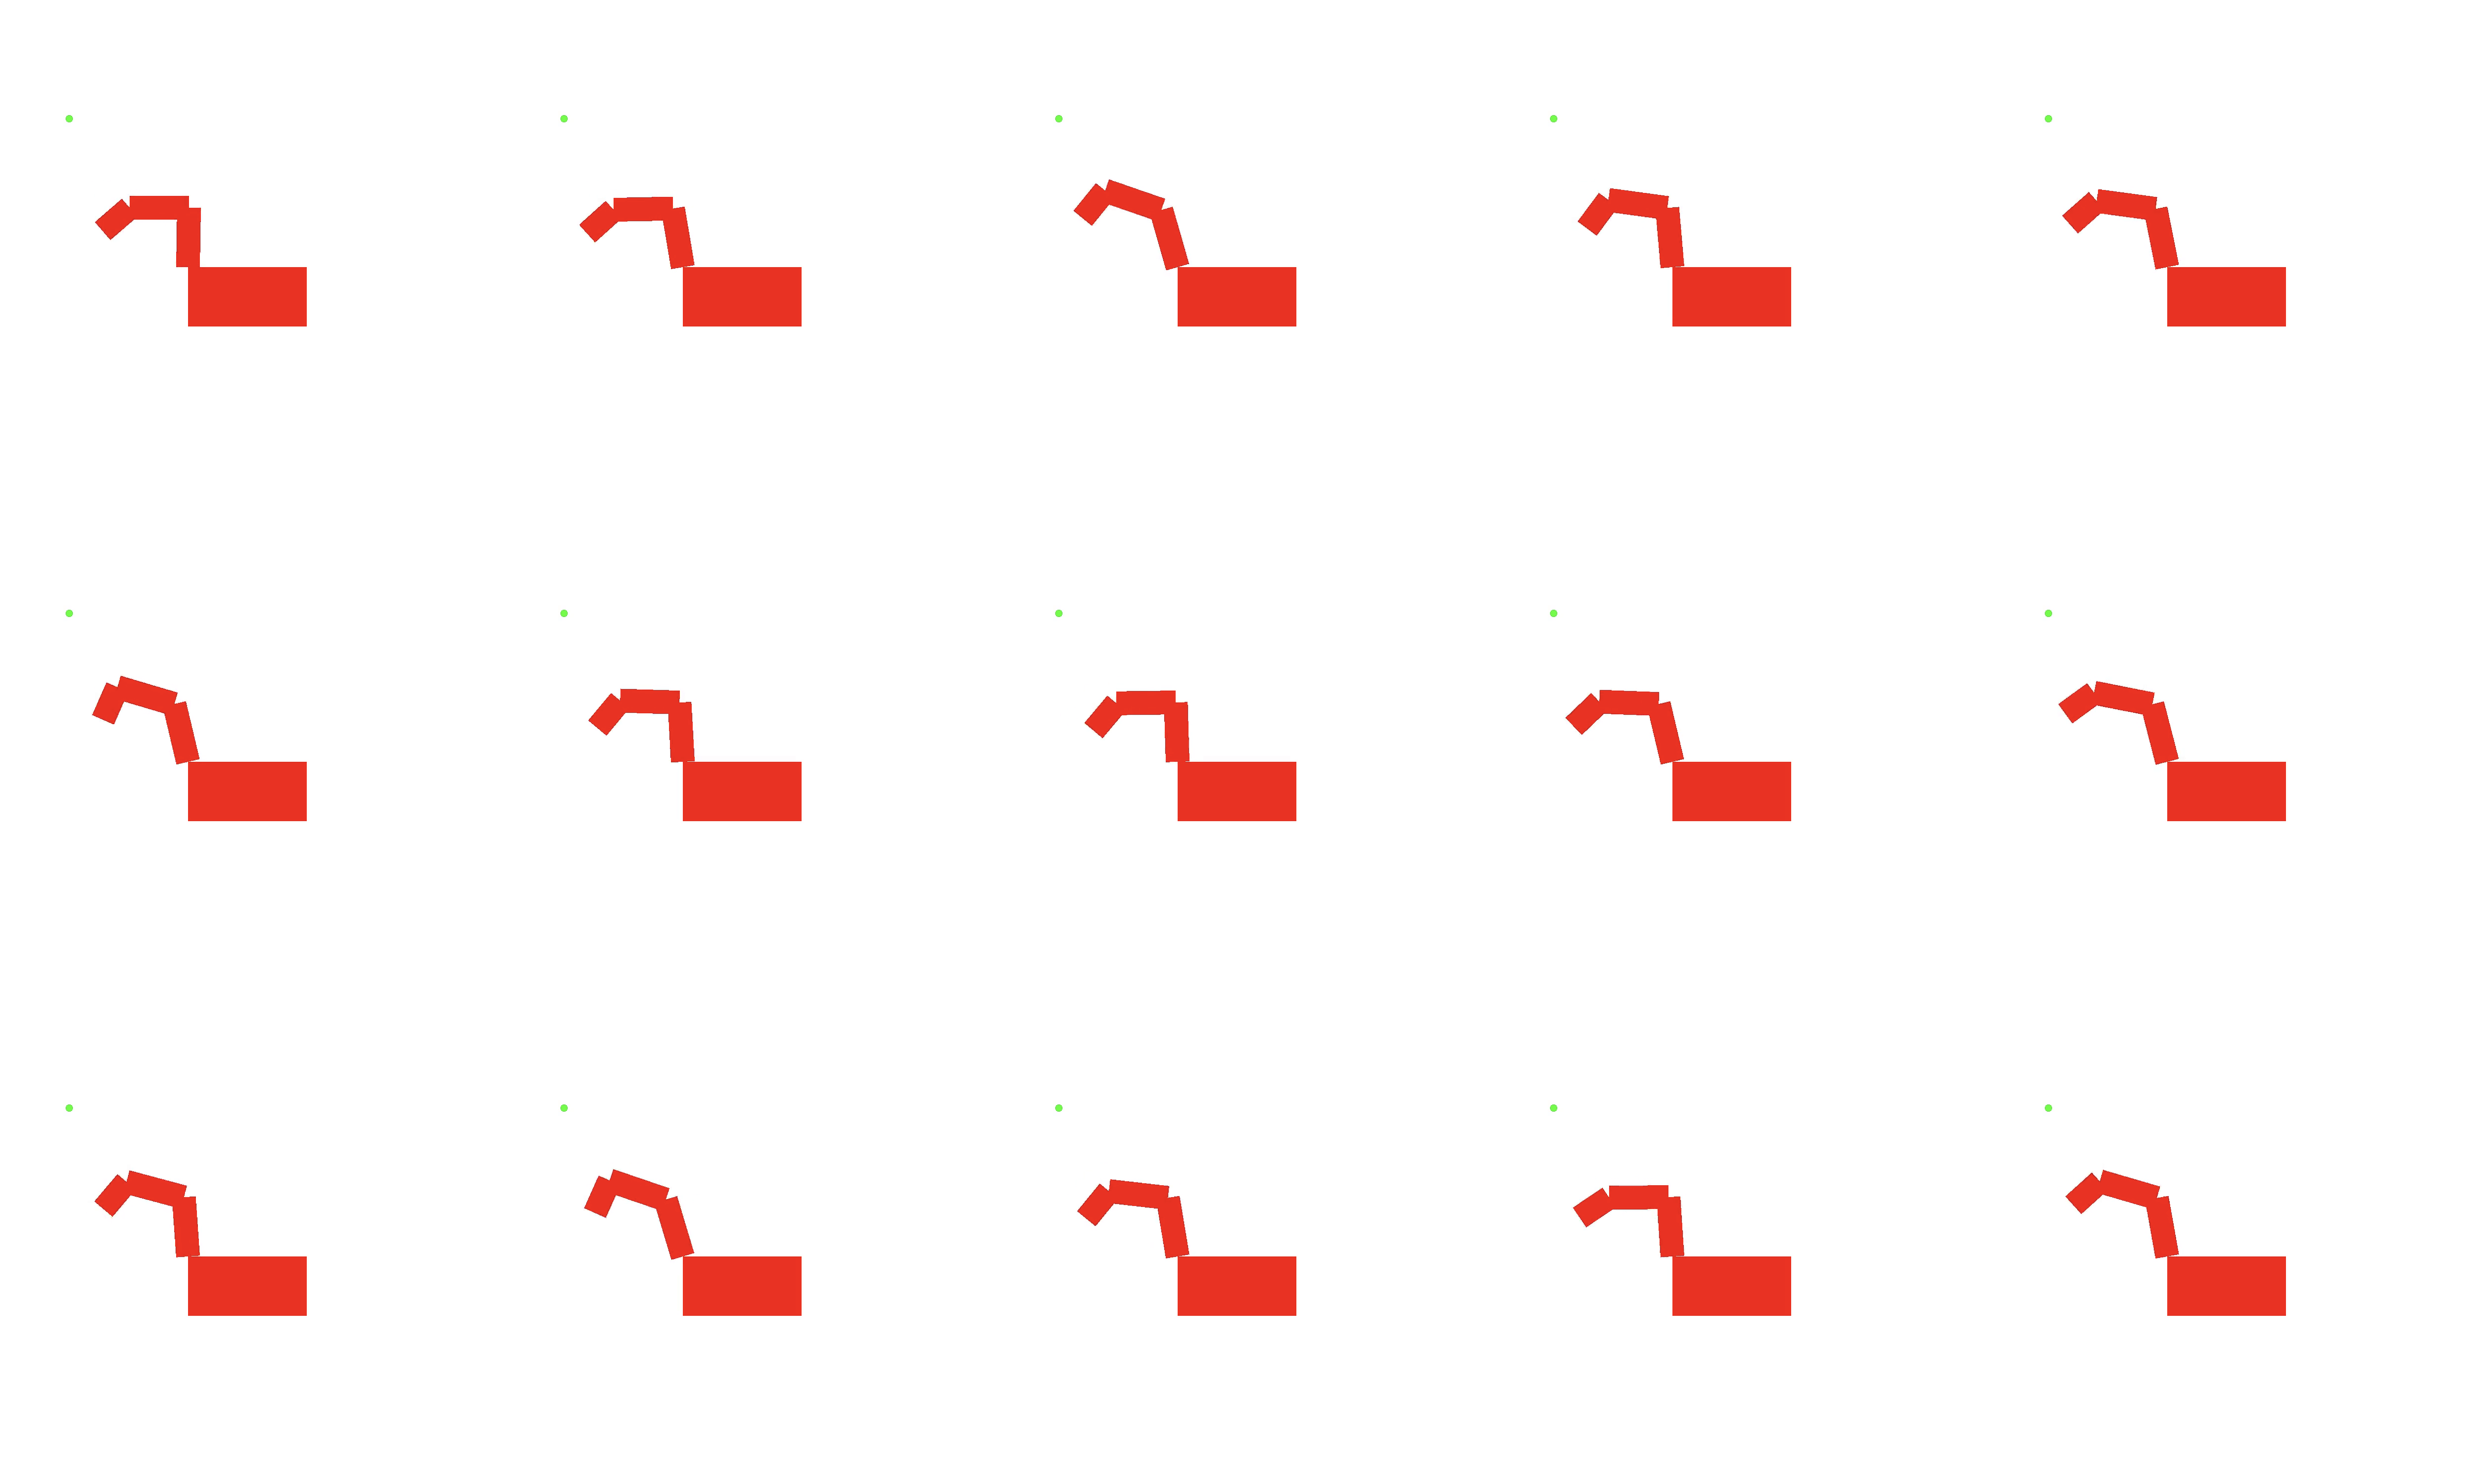
\includegraphics[width=1\textwidth]{figures/frames/frames_004.png}
      \caption{Control of a pigeon model with a static body trained on $r_{fifty\_fifty}$}
      \label{fig:fifty_fifty_body_speed_0}
  \end{figure}

  \begin{figure}[H]
      \centering
      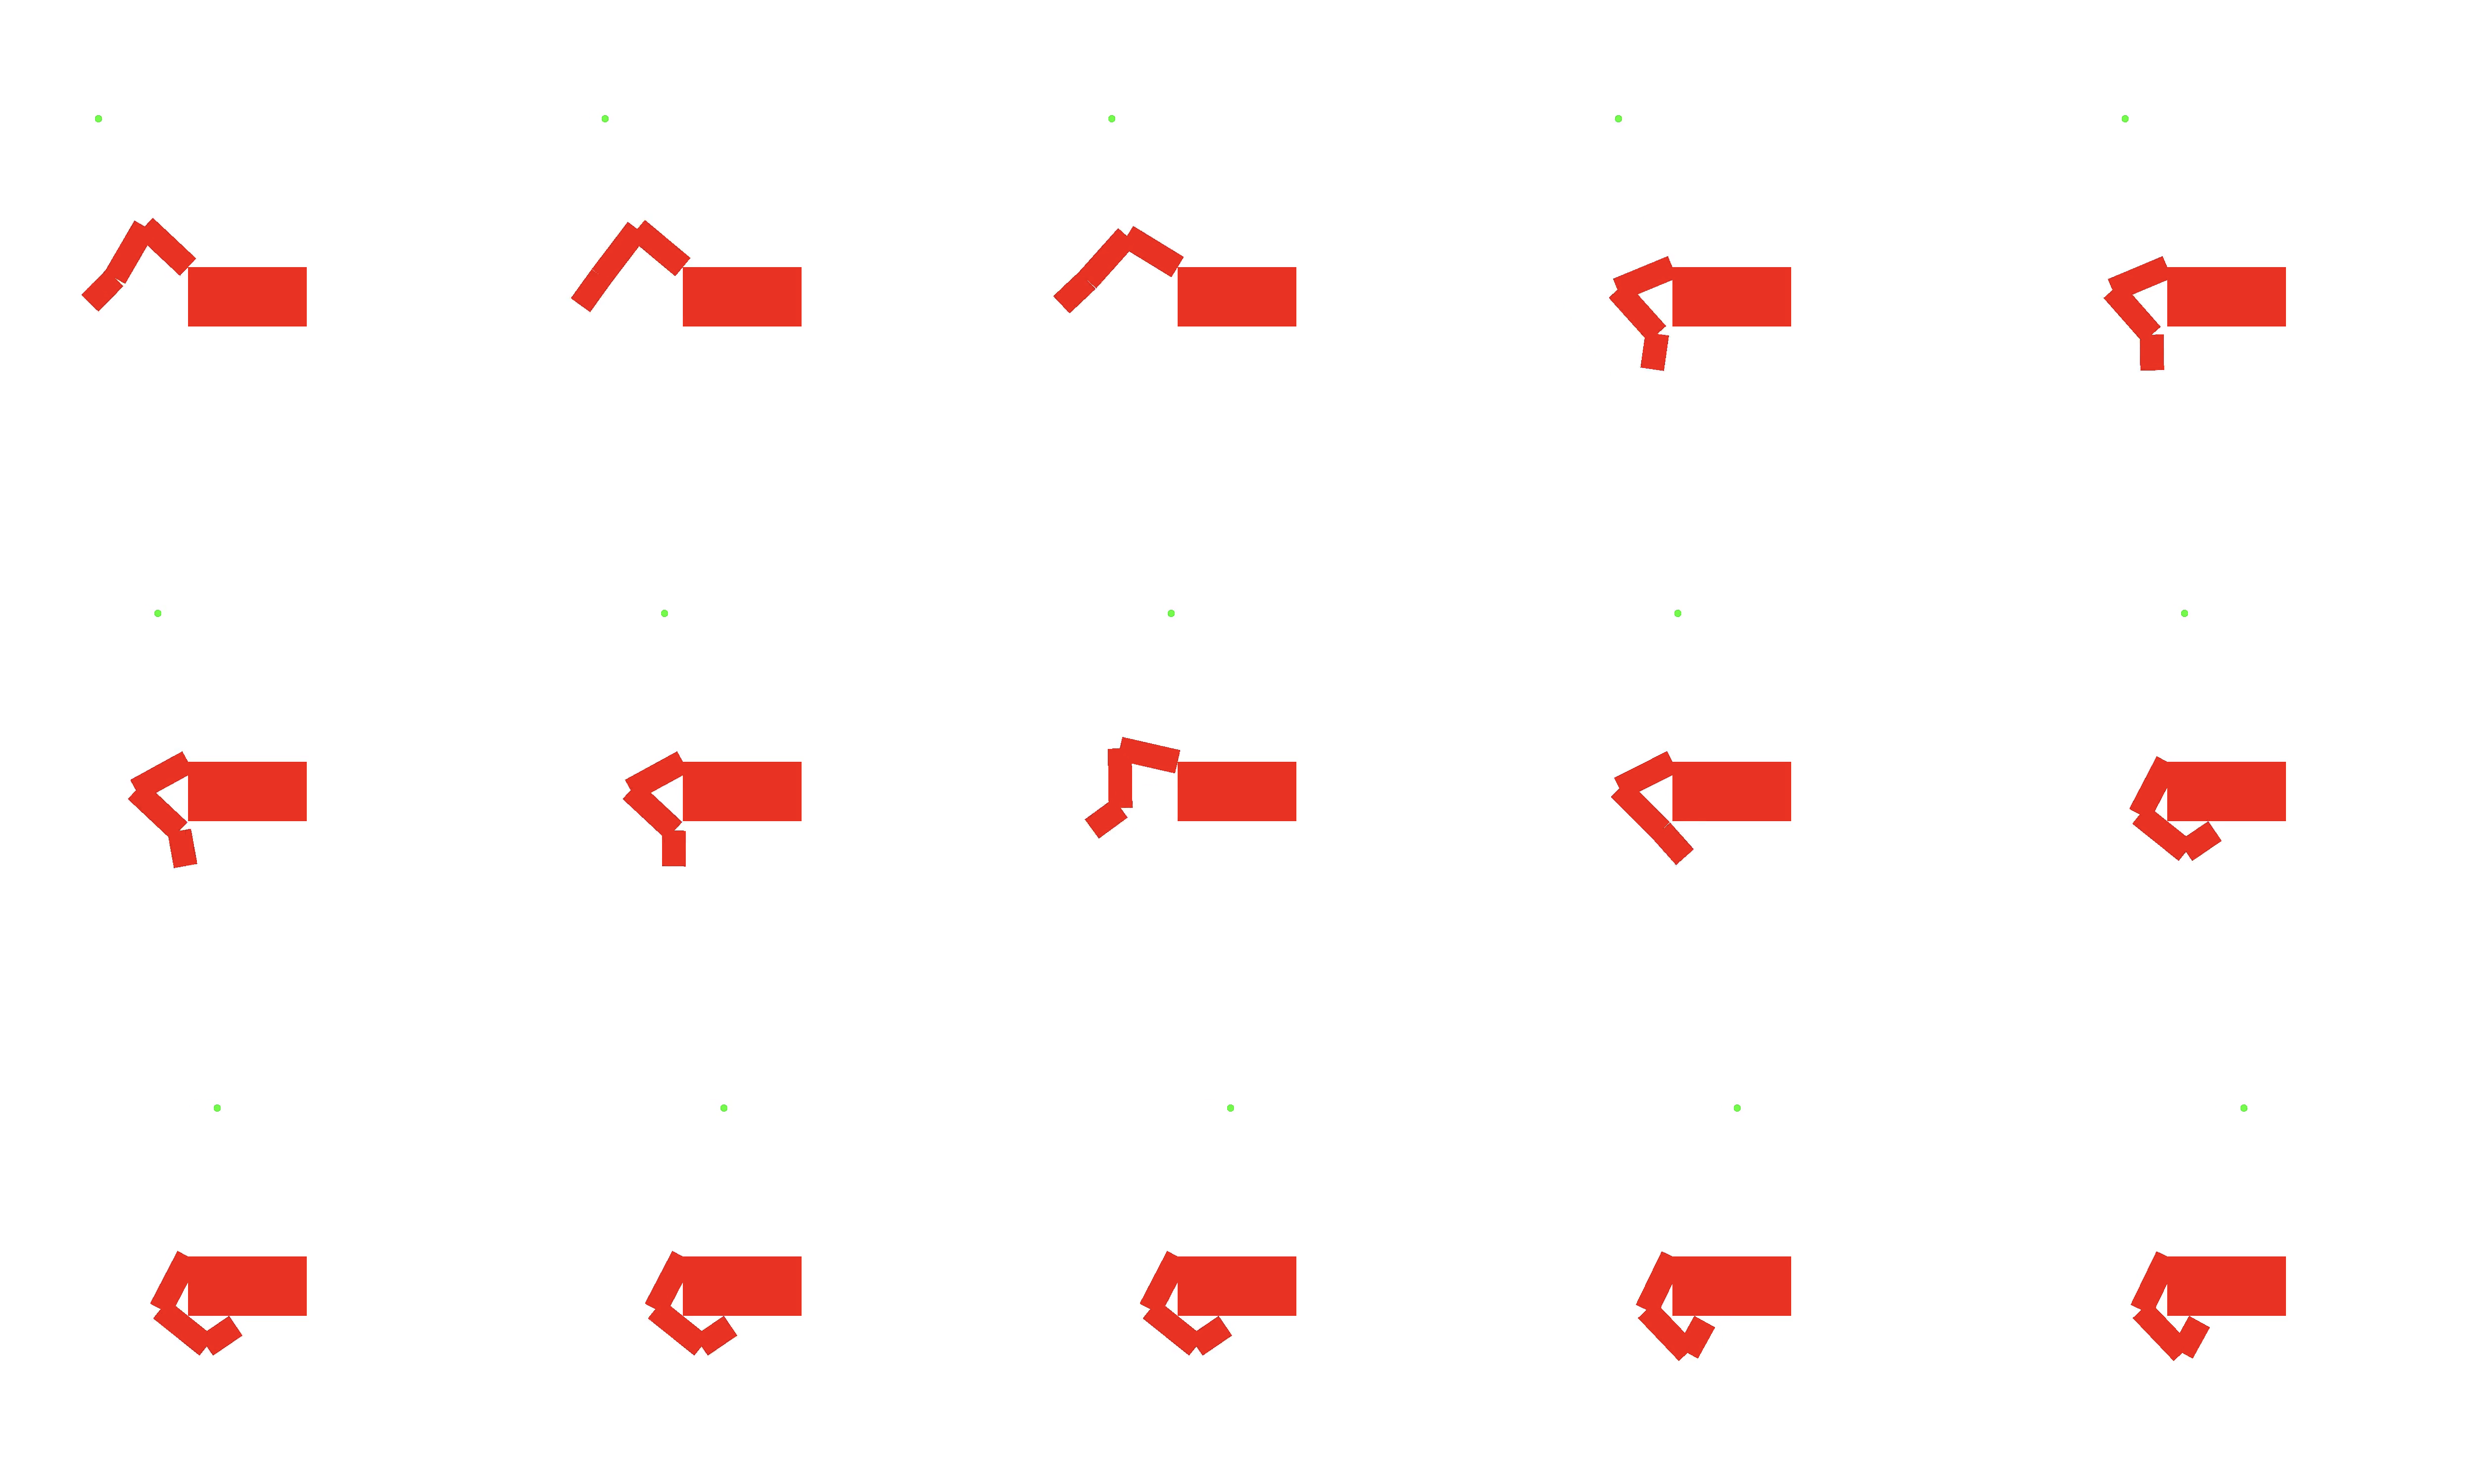
\includegraphics[width=1\textwidth]{figures/frames/frames_005.png}
      \caption{Control of a pigeon model with the body speed of 1 trained on $r_{fifty\_fifty}$}
      \label{fig:fifty_fifty_body_speed_1}
  \end{figure}
